\section{Knowledge Graph Lifecycle \textcolor{red}{-- By 16/2}}
\label{sec:chp2_kg_lifecycle}

%\ana{repasar un poco los papers que hablen de ciclo de vida de KGs, dónde encajan los mappings ahí y qué se ha estudiado en su intervención en el proceso, para decir que en la evolución no se ha estudiado}

%\ana{de aquí lo que se quiere destacar es qué hueco cubrimos: el rol de declarative approaches en evolución de KG. Enmarcado en el KG life cyle, se ha estudiado cómo mejora su construcción y evaluación (randles); pues esto iría en otra etapa del lyfe cycle que no está estudiada hasta ahora}

%\textit{Primera parte: un overview de los lyfe cycles/dev processes propuestos hasta ahora? Comentar las fases comunes, y decidirse por una: que sería una mezcla entre umut's y groth's. Las aprtes que interesan al final van a ser la de knowledge creation/KGconstruction; y la iteración en el mantenimiento, porque son las que involucran los declarative approaches pero se pueden comentar más.  }


A high number of knowledge graphs has been released over the years. Along with this adoption, the question arose about which is are processes involved in their life cycle.
\cite{ngomo2014LD-lifecycle} proposed a series of steps that define the life cycle of Linked Data (\cref{fig:chp2_LD-lifecycle}), the term used at the time for referring to knowledge graphs before this term was coined with the release of the Google knowledge graph\footnote{\url{https://blog.google/products/search/introducing-knowledge-graph-things-not/}}. 
These steps include 
(i) \textit{Extraction} of information from (semi-)structured and unstructured data sources mapping them to an RDF schema; 
(ii) \textit{Storage and Querying} of the graph in a graph store; 
(iii) \textit{Authoring} for users to create, modify or extend the information in the graph;
(iv) \textit{Linking} to external related resources;
(v) \textit{Enrichment} with higher-level structures to aggregate and query data more efficiently;
(vi) \textit{Quality Analysis} to assess the quality of the published data;
(vii) \textit{Evolution and Repair} to address issues and errors detected;
(viii) \textit{Search, Browse and Exploration} for users to navigate the graph in a user-friendly manner. 

\begin{figure*}[]
\centering
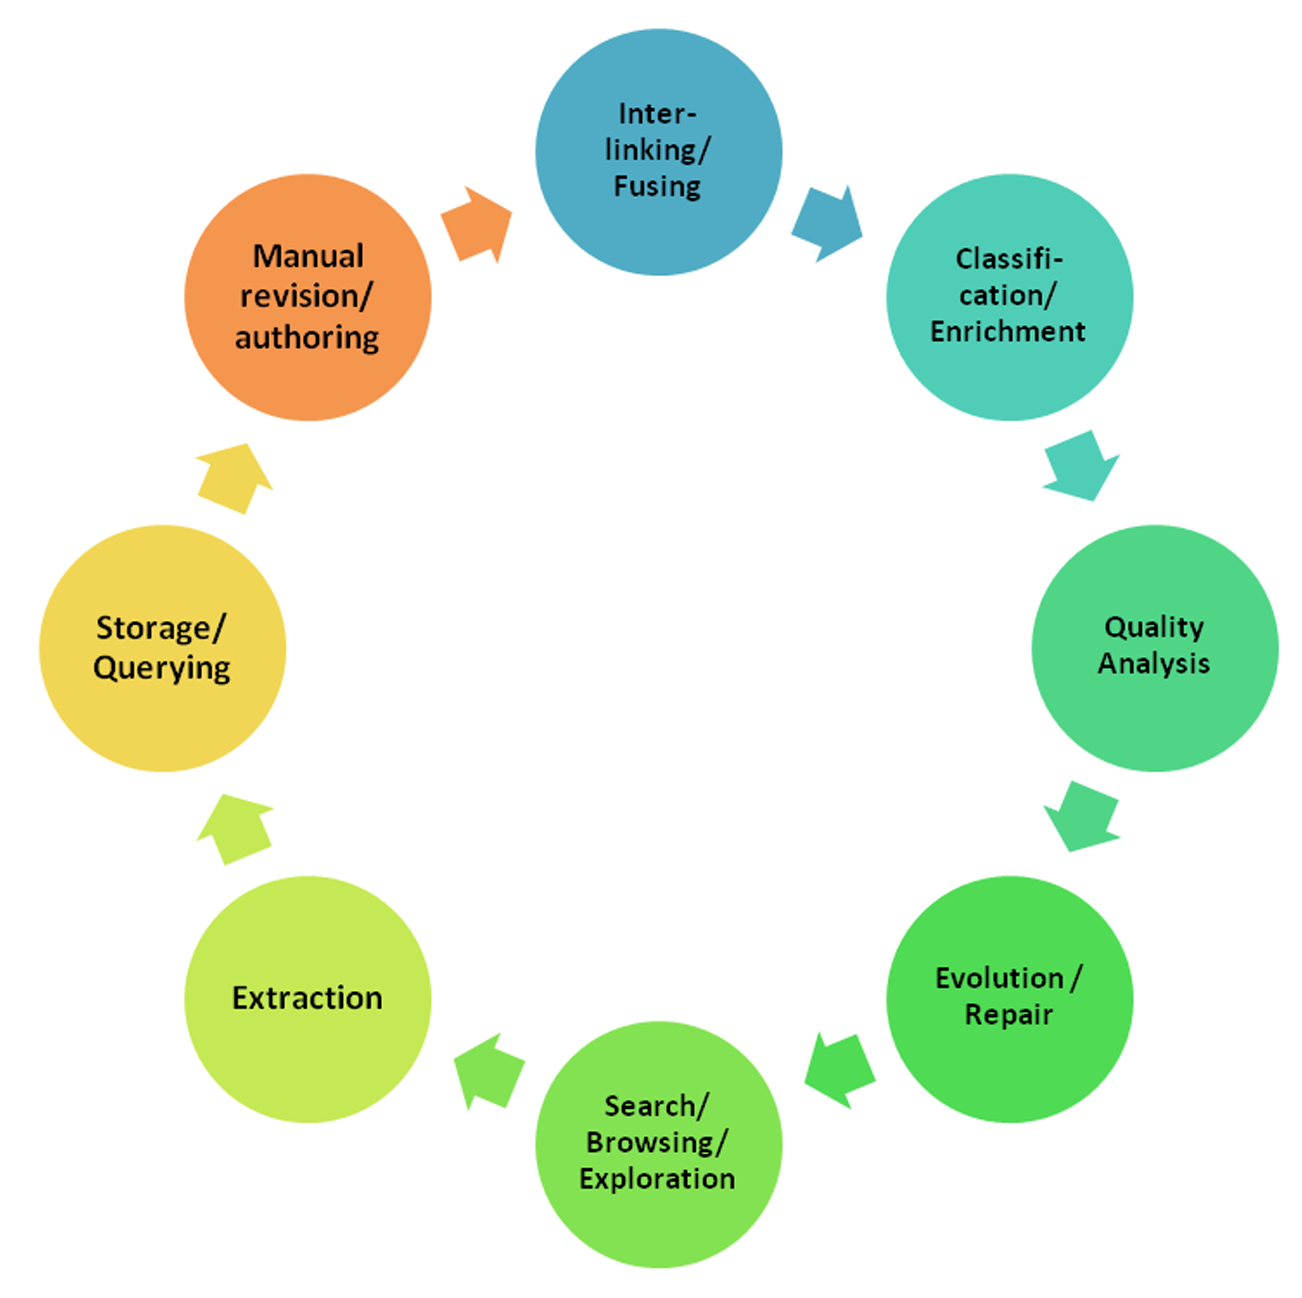
\includegraphics[width=0.6\linewidth]{figures/chp2_LD-lifecycle.png}
\caption{Linked Data life cycle proposed by \cite{ngomo2014LD-lifecycle}.}
\label{fig:chp2_LD-lifecycle}
\end{figure*}

\cite{simsek2021knowledge} proposed a life cycle for knowledge graphs based on the authors' experience, considering a series of steps and iterations (\cref{fig:chp2_lifecycle-Simsek}). The life cycle starts with the 
(i) \textit{Knowledge Creation} to construct the knowledge graph from heterogeneous data sources, followed by the 
(ii) \textit{Knowledge Hosting} in an appropriate graph store. 
Then, the (iii) \textit{Knowledge Curation} cycle takes place, which is comprised of three steps. First, the \textit{Knowledge Assessment} of the quality (considering completeness and correctness) of the knowledge graph, which triggers the other two steps: \textit{Knowledge Cleaning} for error detection and correction, \textit{Knowledge Enrichment} with related resources. 
Once the \textit{Knowledge Assessment} is satisfactory and the knowledge graph is curated, the (iv) \textit{Knowledge Deployment} stage takes place to publish the knowledge graph and make it available for consumption.

\begin{figure*}[]
\centering
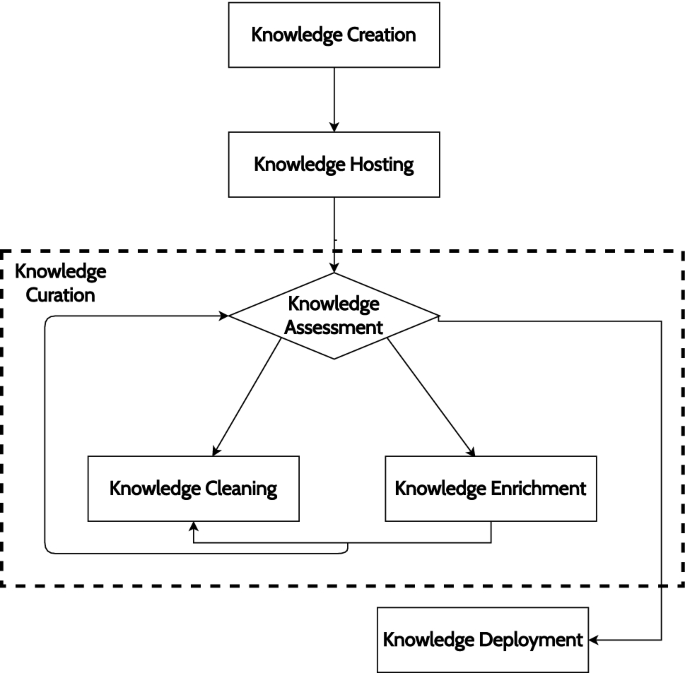
\includegraphics[width=0.5\linewidth]{figures/chp2_lifecycle-Simsek.png}
\caption{Knowledge graph life cycle proposed by \cite{simsek2021knowledge}.}
\label{fig:chp2_lifecycle-Simsek}
\end{figure*}

\cite{tamavsauskaite2023defining} carried out a systematic literature review to find the common stages of Knowledge Graph management process analysing several papers that have described the process followed for their knowledge graphs (\cref{fig:chp2_kg-dev-process}). This process include  
(i) \textit{Identification of data} and domain of interest of the knowledge graph;
(ii) \textit{Construction of the ontology} whenever there is no suitable ontology available;
(iii) \textit{Extraction of knowledge} from the identified data, and more specifically, extracting entities, relations between them and their attributes;
(iv) \textit{Processing of knowledge} to ensure its high quality, which involves integration from different sources, cleaning, mapping to the ontology, completion, enrichment and validation;
(v) \textit{Knowledge graph construction} to store it and make it available and accessible for consumption;
and (vi) \textit{Knowledge graph maintenance} for evaluating the knowledge graph quality and updates for evolution.


\begin{figure*}[]
\centering
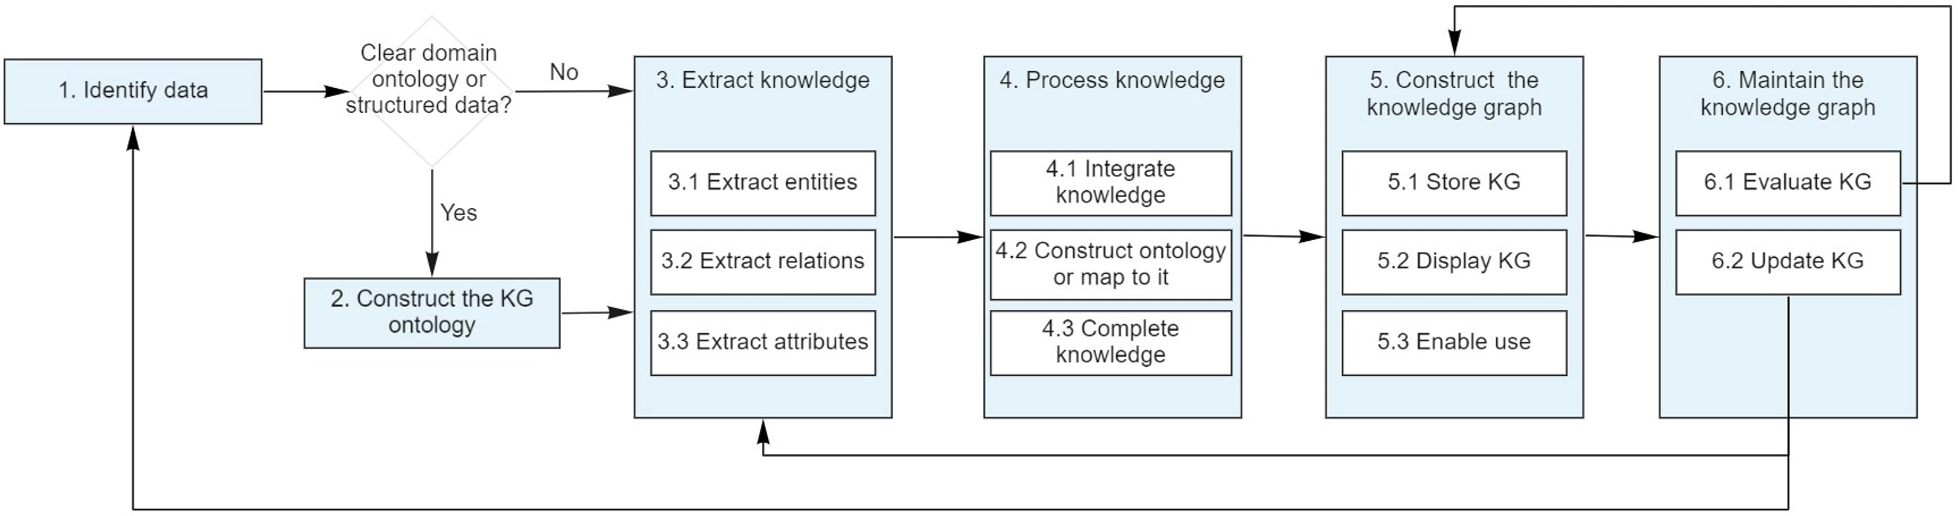
\includegraphics[width=\linewidth]{figures/chp2_kg-dev-process.png}
\caption{Knowledge graph development proposed by \cite{tamavsauskaite2023defining}.}
\label{fig:chp2_kg-dev-process}
\end{figure*}

\textit{All these proposed life cycles have stages in common or consider similar aspects. Declarative approaches are in the end involved in the construction, and there are several studies analysing how they can improve or enhance this step? }

\textit{ºcontinuando con la de antes: enmarcado dentro de este life cycle dónde intervendrían los mappings: en la creación y en cada iteración que haya que hacer (cuadra más groth's aquí eso sí). Señalar paper de benchmark de todas las fases en algún momento. Dentro de la creación de cero, por supuesto porque esa es su función principal. Ahí qué hay de mejora: el de bio2rdf contra php, y todas las optimizaciones del proceso, comentar si acaso del paper de vir vs mat de dylan si está publicado. }

\textit{Mirar si randles et al ha mirado algo de quality gracias a mappings; y comentar si es así. Si no se señala el gap en cómo pueden intervenir estos approaches en más fases, por ej en la evolución.}
